\section{Experiments}

We present various mathematical expressions, which can be computed more efficiently
than initial formulation would suggest. 

\subsection{Matrix Multiplication-Sum Identities}

Given matrices $A \in \mathbb{R}^{n \times m}$, $B \in \mathbb{R}^{m
  \times k}$, we wish to compute:
\begin{gather*}
\sum AB = \sum_{i = 1}^n \sum_{k = 1}^m \sum_{j = 1}^k A_{i, k} B_{k, j} 
\end{gather*}
A naive algorithm would take $O(nmk)$ time. However, we have found with our framework 
computation giving the same expression in time $O(n(k + m))$:
\begin{lstlisting}
sum(sum(A .* repmat(sum(B, 2), [1, m])'))
\end{lstlisting}
Empirical tests indicate that our expression is indeed faster to
compute than the naive one (Figure \ref{ab}).

\begin{figure}[h]
\centering
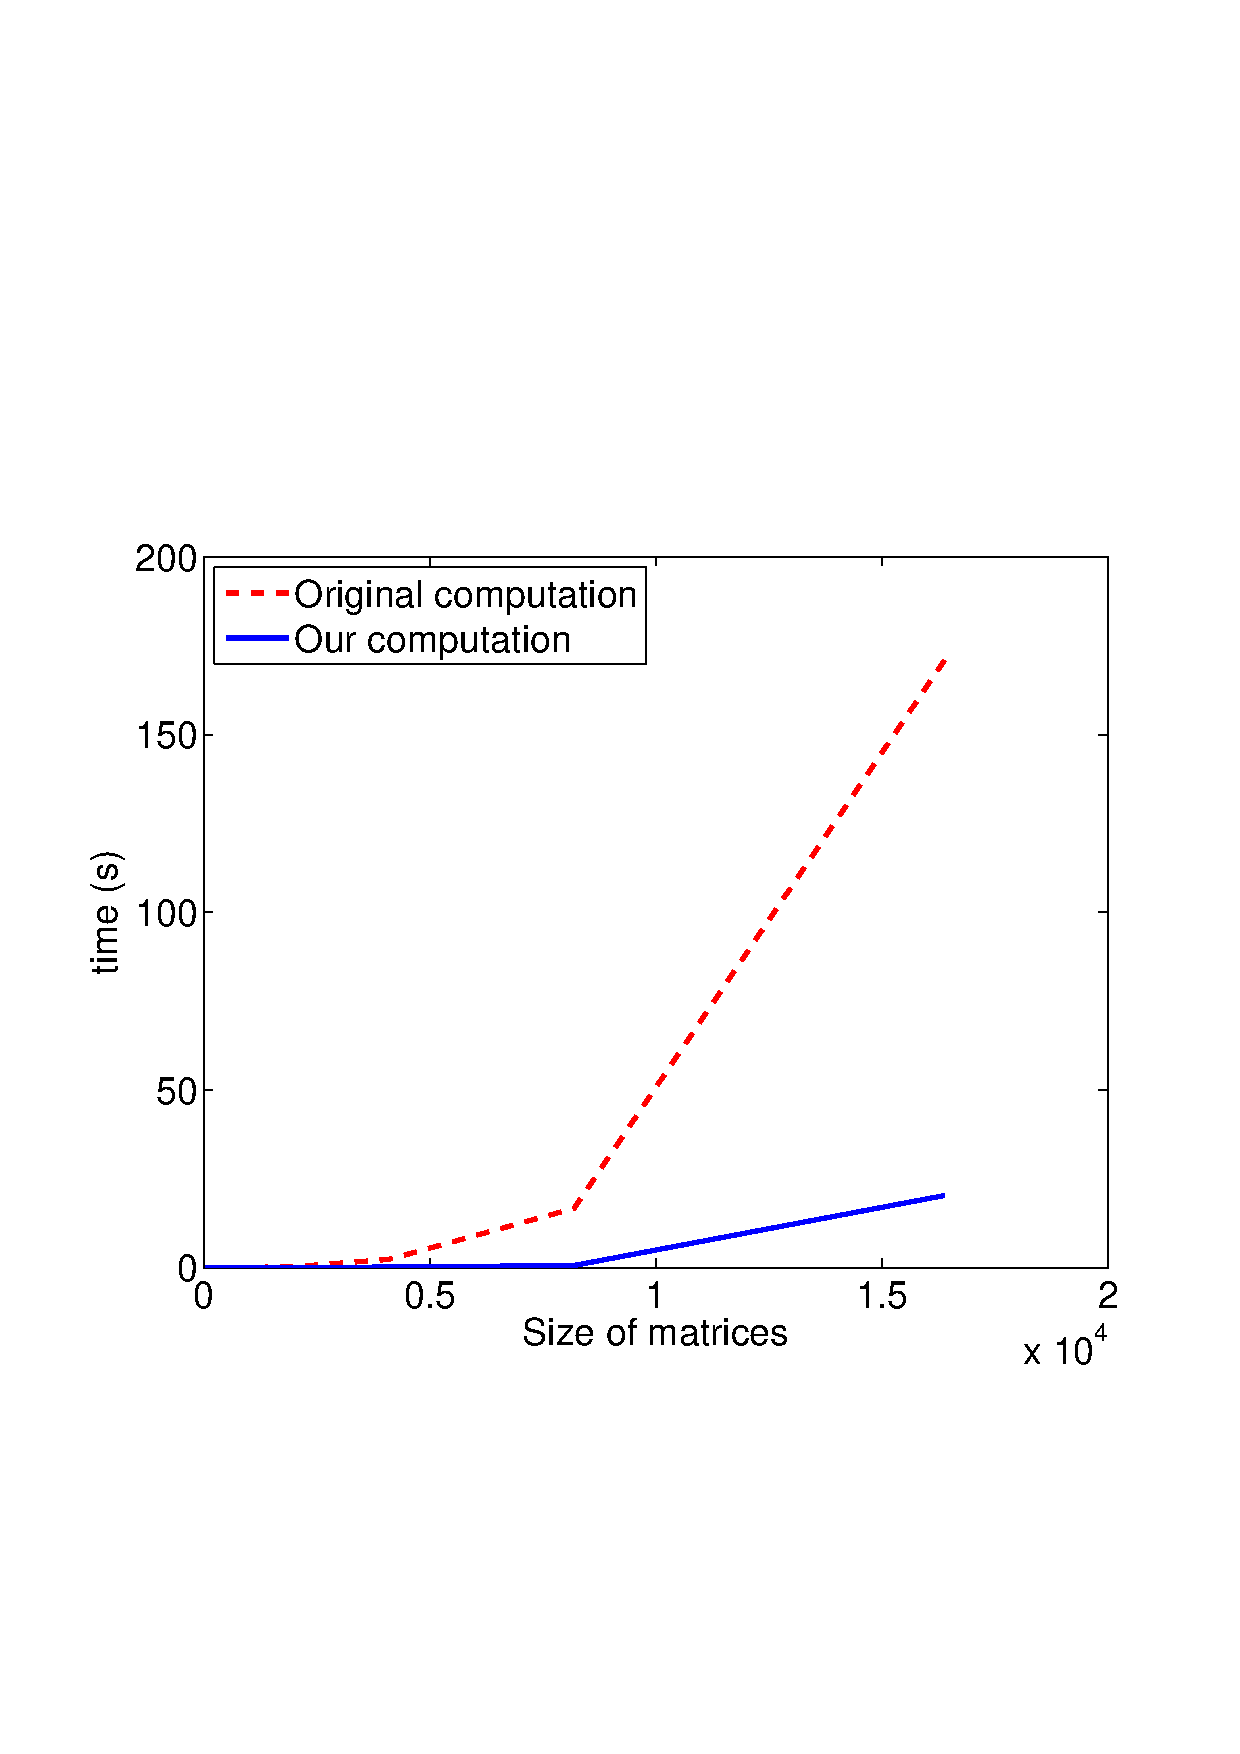
\includegraphics[scale=0.3]{img/ab.png}
\caption{Computation time for $\sum AB$ using standard algorithm vs using inferred optimal algorithm.}
\label{ab}
\end{figure}

Similarly, we found quadratic time computation, instead of cubic, for
similar expressions such as: 
\begin{align*}
	\sum ABC\text{, }\sum ABCD\text{, }\sum AA^T\text{, }\sum AA^TA
\end{align*}

As far we we are aware, these identities appear to be novel. Our
system could automatically analyze large code repositories to find
these and other expressions, which are currently computed
inefficiently. Alternativeily, our optimization rules could be placed
into compilers to generate efficient code.

\subsection{Partition Function Approximation}

As we showed in Section \ref{partitionfunction}, we can manually find
$O(n^2)$ computation of $g(x \rightarrow x^k, W)$ for $k = 1, 2$
instead of native exponential time computation. By use of our
framework, we found rules for $k = 3, 4, 5$. However for $k = 4, 5$
these rules used computation with $O(n^3)$ time (i.e.~matrix
multiplication).  Finding computational rules for higher degree
polynomials is expensive: Table \ref{grammars} shows the time
necessary to generate all the rules. It is worth noting that grammar
can be evaluated just once, and the resulting coefficients can be
stored. Furthermore, the process of discovering the computational rule
for a given power only need to be performed once. However, due to limited computational
power we analyzed only powers $k \leq 5$. As we note in Section
\ref{agenda} a future direction would be to learn patterns for
$k=2,3,4,5$ that allow us to generalize to $k>5$ without exhaustively
searching all possible rules. 

Table \ref{eval} shows number of terms necessary to derive $g(x
\rightarrow x^k, W)$ for various $k$. Figure \ref{approximations} shows
how well partition function is approximated with finite Taylor
expansion. Finally, Figure \ref{time_approx} compares computation time
of derived rules to the computation time of naive exponential time
algorithm.

\begin{table}
\tiny
\centering
\begin{tabular}{rrr}
\hline
Degree & Grammar size & Time (s) \\
\hline
2 & 5 & 17 \\
3 & 15 & 188 \\
4 & 48 & 2535\\
5 & 139 & 31320 \\
\hline
\end{tabular}
\caption{Table summarizes size and computational time for grammars of specific degree. 
All computation here are performed on expressions, and have nothing to do with computation time on instantiations.
This procedure has to be executed only once.}
\label{grammars}
\end{table}

% TODO(wojciech): \mathbf was on purpose below? it's not consistent.
% TODO(karol): we need more columns in those tables, or we should consider merging them
\begin{table}
\tiny
\centering
\begin{tabular}{rrr}
\hline
Degree & Num. terms & Complexity \\
\hline
2 & 4 & $O(n^2)$\\
3 & 5 & $O(n^2)$\\
4 & 21 & $\mathbf{O(n^3)}$\\
5 & 30 & $\mathbf{O(n^3)}$\\
\hline
\end{tabular}
\caption{Table summarizes complexity of computation of $g(x \rightarrow x^k, W)$. 
Number of terms, and complexity of every term is important for the computation of the target expression.
Potentially, we need to evaluate partition function multiple times, so the ``Complexity''
is the complexity of our final system were we use such expressions.} 
\label{eval}
\end{table}

\begin{figure}[h]
\centering
\includegraphics[scale=0.2]{img/approximations.png}
\caption{Comparison of approximations with various number of Taylor terms.}
\label{approximations}
\end{figure}



\begin{figure}[h]
\centering
\includegraphics[scale=0.24]{img/time_approx.png}
\caption{Comparison of computation time for naive exponential time algorithm vs our optimized derivation.}
\label{time_approx}
\end{figure}


